\documentclass[dvipdfmx,10pt,a4paper,titlepage]{jsarticle}
\usepackage[dvipdfmx]{graphicx}
\usepackage{ascmac}
\usepackage{amsmath}
\usepackage{fancybox}
\usepackage{amssymb}
\usepackage{mathtools}
\usepackage{latexsym}
\usepackage{listings,jvlisting}
\usepackage{color}
\usepackage{url}
\definecolor{OliveGreen}{rgb}{0.0,0.6,0.0}
\definecolor{Orenge}{rgb}{0.89,0.55,0}
\definecolor{SkyBlue}{rgb}{0.28,0.28,0.95}
\lstset{
  basicstyle={\ttfamily},
  identifierstyle={\small},
  commentstyle={\small\itshape},
  keywordstyle={\small\bfseries},
  ndkeywordstyle={\small},
  stringstyle={\small\ttfamily},
  frame={tb},
  breaklines=true,
  columns=[l]{fullflexible},
  numbers=left,
  xrightmargin=0zw,
  xleftmargin=3zw,
  numberstyle={\scriptsize},
  stepnumber=1,
  numbersep=1zw,
  lineskip=-0.5ex,
  keepspaces=true,
  keywordstyle={\color{SkyBlue}},
  commentstyle={\color{OliveGreen}},
  stringstyle=\color{Orenge},
  showstringspaces=false
}
\title{マイクロプロセッサの設計と実装 最終レポート}
\author{
    東京大学電子情報工学科3年\\
    03230422 佐藤 龍吾
}
\date{\today}

\begin{document}
    \maketitle
    \section{設計方針・実験日程}
    本実験では、10日間でRISC-VのマイクロプロセッサをVerilogで記述し、FPGA上でテスト、CoreMarkを用いたベンチマークを行った。
    表~\ref{tab:day}のスケジュールで実験を行った。実装過程はGitLab\footnote{\url{https://exp.mtl.t.u-tokyo.ac.jp/SugarDragon5/b3exp}}で管理した。

    本実験での開発目標を「CoreMarkスコア3桁」とし、効率的な開発のために以下の点に意識した。
    \begin{itemize}
        \item 各モジュールの仕様や、モジュール間のやり取りのフロー・タイミングを実装前に極力明確にし、実装時はその通り書くだけで済むまで考察した。
        \item 必要なモジュールや機能をissueに切り出して管理することで、進捗の把握を容易にし、次に実装するべき機能を明確にした。
        \item 各テストやCoreMarkの実装が最低限のコマンドで済むよう、コンパイルから実行までをシェルスクリプトでまとめた。
        \item 終盤まで細かいチューニングは行わず、新規機能の実装に集中した。
        ただし、直前の実装に比べ大幅に周波数が下がらないよう最低限のチューニングは行った。
        \item GitHub Copilotを駆使し、ALU, Decoderのような単純作業の繰り返しを半自動・高速に行った。
        AIの補完を利用した部分はバグになりがちなので、Copilotの提案内容はすべて一言一句確認し、自分の想定したプログラムと違わないかを確認した。
    \end{itemize}
    \begin{table}[h]
        \begin{center}
            \caption{実験日程}\label{tab:day}
            \begin{tabular}{l|l}
                日付 & 実装内容 \\ \hline
                Day 1(10/31) & ALUの実装 \\
                Day 2(11/2)  & シングルサイクルプロセッサの実装 \\
                Day 3(11/6)  & 5ステージ化・シミュレーションテスト \\
                Day 4(11/7)  & CoreMarkデバッグ \\
                Day 5(11/9)  & CoreMark完動 \\
                Day 6(11/13) & パイプライン化実装 \\
                Day 7(11/14) & パイプライン化実装・完動 \\
                Day 8(11/16) & 分岐予測実装 \\
                Day 9(11/20) & 周波数チューニング \\
                Day 10(11/27)& RV32M命令実装・発表
            \end{tabular}
        \end{center}
    \end{table}
    \section{実装内容・アーキテクチャ}
    Day 5に完成したv1.0から、Day 10に完成したv4.1まで、計7つのバージョンを作成した。
    バージョンごとに、実装内容とアーキテクチャ、工夫した部分やアルゴリズムについてまとめる。

    また、各バージョンに対応するCommitはGitLab上でタグを付けてある。\url{https://exp.mtl.t.u-tokyo.ac.jp/SugarDragon5/b3exp/-/tags}
    \subsection{v1.0}
    \subsubsection{実装内容}
    v1.0では、RV32I対応の最小限のプロセッサを実装した。
    パイプライン化を念頭に置き、IF(Instruction Fetch)、RR(Register Read)、EX(Execute)、MA(Memory Access)、RW(Register Write)の5ステージに分け、1命令に付き5クロックで実行するようにした。
    各ステージの機能は
    \begin{itemize}
        \item IFステージ: PCをもとにROMから命令をフェッチする。
        \item RRステージ: IFステージでフェッチした命令をデコードし、レジスタからオペランドを読み出す。
        \item EXステージ: RRステージでデコードした命令を実行する。
        \item MAステージ: EXステージで実行した命令がメモリアクセスを必要とする場合、メモリアクセスを行う。
        \item RWステージ: EXステージの計算結果 / MAステージのメモリアクセス結果をレジスタに書き込む。
    \end{itemize}
    モジュールのうち、ROM, RAM, Register File (書き込み), ALU, Decoderはクロックの立ち上がりで動作するようにし、それぞれ動作させたいときは前クロックで同期リセット入力を渡した。
    アーキテクチャ図としては、図~\ref{fig:v1.0}のようになる。
    \begin{figure}[h]
        \centering
        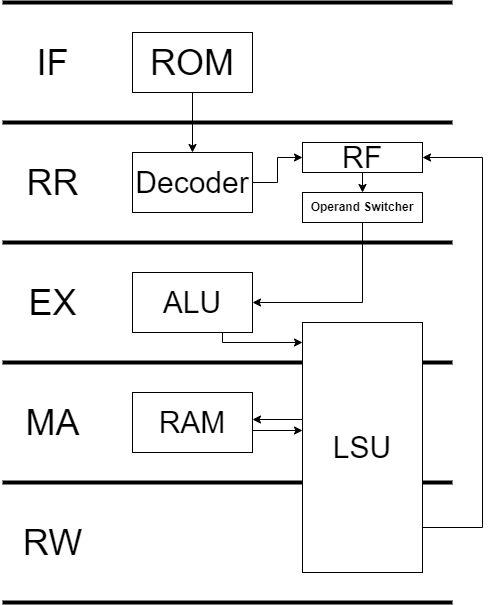
\includegraphics[width=7cm]{figure/v1.0.png}
        \caption{v1.0のアーキテクチャ図}\label{fig:v1.0}
    \end{figure}
    \subsubsection{パフォーマンス}
    Vivadoを用いて合成したところ、最大クロック周波数は$80\mathrm{MHz}$付近となった。
    FPGA上で$80\mathrm{MHz}$でCoreMarkを動作した結果は表~\ref{tab:v1.0}の通りである。
    \begin{table}[h]
        \begin{center}
            \caption{v1.0のCoreMark結果}\label{tab:v1.0}
            \begin{tabular}{ll}
                CoreMark & 23 \\
                CoreMark / MHz & 0.288 \\
                IPC & 0.199 \\
            \end{tabular}
        \end{center}
    \end{table}
    5クロックで1命令を処理するので、IPCが約0.2となった。
    \subsection{v2.2}
    \subsubsection{実装内容}
    v2台はv1台のプロセッサをベースにパイプライン化を行ったものである。v2.2では、v1.0同等の処理を行うIF, ID(Instruction Decode),EX, MA, RWの5ステージに分割し、
    各ステージで1命令ずつ処理を行うようにした。このパイプラインを正確に実装する上で、次の点に注意した。
    \begin{itemize}
        \item 1クロックに付き1つの命令をフェッチする必要があり、フェッチした命令をデコードする前に次の命令のPCを計算する必要がある。
        分岐命令かどうか・分岐するかどうかがわからない状態なので、とりあえず分岐しないと仮定し、PC+4を次の命令のPCとした。
        分岐が発生するかどうかはEXステージで確定し、正しいPCとIDステージで動作しているPCが一致しない場合、IFステージ・IDステージの内容を破棄し、次クロックでは正しいPCから命令をフェッチするようにした。
        (以降このケースを「分岐失敗」とよび、破棄の必要がなかった場合を「分岐成功」と呼ぶ)
        \item 連続する命令$I_1, I_2$について、$I_1$でレジスタ$r$に書き込み、$I_2$で$r$から読み込むとき、
        $I_2$がレジスタで読み込む時点では$I_1$の書き込みが完了していないため正しい値が読み込まれない。
        $I_1$で書き込む正しい値が確定するのは、Load命令の場合MAステージ、それ以外ではEXステージである。
        したがって、Load命令以外はEXステージからフォワーディングを行い、
        Load命令は1クロックのストールを行ってからフォワーディングを行うことで解消した。
    \end{itemize}
    
    また、v1台ではROM, RAMともに分散RAMで推論されていたが、v2.1で修正を行い、ROM, RAMともにブロックRAMで推論されるようにした。
    読み出しをクロック同期にしなければいけないが、読み出し先のアドレスはクロックの立ち上がりで代入されるため、ROM、RAMの動作はクロックの立ち下がりで行うようにした。

    \subsubsection{パフォーマンス}
    Vivadoを用いて合成したところ、最大クロック周波数は$70\mathrm{MHz}$付近となった。
    FPGA上で$70\mathrm{MHz}$でCoreMarkを動作した結果は表~\ref{tab:v2.2}の通りである。
    \begin{table}[h]
        \begin{center}
            \caption{v2.2のCoreMark結果}\label{tab:v2.2}
            \begin{tabular}{ll}
                CoreMark & 68 \\
                CoreMark / MHz & 0.971 \\
                IPC & 0.697 \\
                分岐成功率 & 85.73\% \\
            \end{tabular}
        \end{center}
    \end{table}
    パイプライン化により1クロックあたり1命令の処理が可能であり、理想的な命令列の場合のIPCは1となる。
    分岐が失敗するたびに図~\ref{fig:predictfail}のように2命令・10ステージ分の無駄が発生し、IPCが低下する。
    \begin{figure}[h]
        \centering
        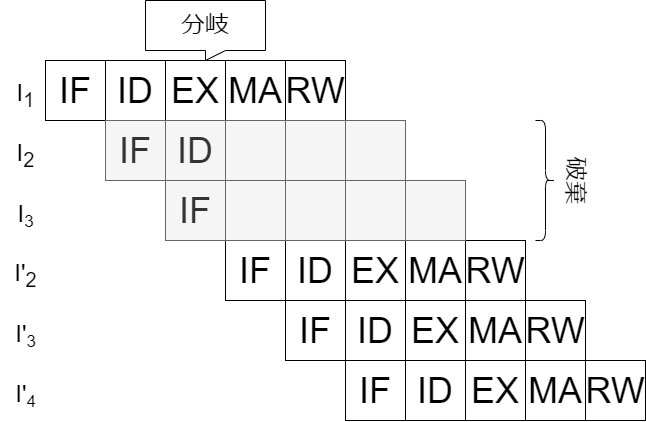
\includegraphics[width=9cm]{figure/predict_fail.png}
        \caption{パイプラインで分岐が失敗したときの挙動}\label{fig:predictfail}
    \end{figure}
    \subsection{v3.0}
    \subsubsection{実装内容}
    v3台はv2台のプロセッサをベースに分岐先予測器を実装したものである。
    v2のプロセッサは分岐命令があるたびに2命令のロスが発生しており、かなり効率が悪い。
    分岐命令に対し正しい分岐先PCを予測し、そこから命令をフェッチできるようにする機構が必要である。

    そこでv3.0では、BTB(Branch Target Buffer)を実装した。
    BTBはPCの一部をキーとしたテーブルで、PC照合用のタグと分岐先PCを格納する。図~\ref{fig:btb}に実装したBTBの構造を示す。
    16bitのPCのうち上位6bitをタグ、残りのうち下位2bitを切り捨てた8bitをインデックスとして用いる。
    このインデックスを用いてBTBのテーブルを検索し、タグが一致した場合、その分岐命令の分岐先PCを返す。
    タグが一致しなかった場合、BTBには分岐先PCが格納されていないと判断し、その命令は分岐分岐命令ではないと判断する。
    
    BTBの書き込みは、EXステージでALUの演算結果として分岐が発生することが判明した際に行う。
    \begin{figure}[h]
        \centering
        \includegraphics[width=12cm]{figure/btb.png}
        \caption{BTBの構造}\label{fig:btb}
    \end{figure}
    \subsubsection{パフォーマンス}
    Vivadoを用いて合成したところ、最大クロック周波数は変わらず$70\mathrm{MHz}$付近となった。
    FPGA上で$70\mathrm{MHz}$でCoreMarkを動作した結果は表~\ref{tab:v3.0}の通りである。
    \begin{table}[h]
        \begin{center}
            \caption{v3.0のCoreMark結果}\label{tab:v3.0}
            \begin{tabular}{ll}
                CoreMark & 78 \\
                CoreMark / MHz & 1.11 \\
                IPC & 0.808 \\
                分岐成功率 & 91.72\% \\
            \end{tabular}
        \end{center}
    \end{table}
    \subsection{v3.1}
    \subsubsection{実装内容}
    v3.1では、v3.0のBTBに加え、PHT(Pattern History Table)を実装した。
    BTBは分岐先のPCを格納するだけで、分岐の成否に関する情報は持っていない。
    Branch命令には分岐頻度が高いもの(ループなど)と低いもの(例外処理)があり、BTBのみでは頻度が低い分岐の予測失敗率が高い。
    したがって、分岐条件が成立するかどうかを記憶・判定する必要がある。

    PHTはBTBと同じくPCの一部をキーとしたテーブルで、分岐条件の成否を格納する。各テーブルは2bitで、
    \begin{itemize}
        \item 00: 分岐しないと強く予測
        \item 01: 分岐しないと弱く予測
        \item 10: 分岐すると弱く予測
        \item 11: 分岐すると強く予測
    \end{itemize}
    の4つの状態を持つ。図~\ref{fig:pht}に実装したPHTの構造を示す。
    BTB同様PCのうち上位6bitと下位2bitを切り捨てた8bitをインデックスとして用い、
    \begin{itemize}
        \item BTBがヒットし、PHTが10か11の場合: BTBの分岐先PCを返す
        \item BTBがヒットしたが、PHTが00か01の場合: 分岐しないと予測し、PC+4を返す
        \item BTBがヒットしなかった場合: 分岐しないと予測し、PC+4を返す
    \end{itemize}
    とする。
    PHTへの書き込みは、BTBと異なり分岐命令以外に対しても行う。
    \begin{figure}[h]
        \centering
        \includegraphics[width=12cm]{figure/pht.png}
        \caption{PHTの構造}\label{fig:pht}
    \end{figure}
    \subsubsection{パフォーマンス}
    Vivadoを用いて合成したところ、最大クロック周波数は変わらず$70\mathrm{MHz}$付近となった。
    FPGA上で$70\mathrm{MHz}$でCoreMarkを動作した結果は表~\ref{tab:v3.1}の通りである。
    \begin{table}[h]
        \begin{center}
            \caption{v3.1のCoreMark結果}\label{tab:v3.1}
            \begin{tabular}{ll}
                CoreMark & 84 \\
                CoreMark / MHz & 1.2 \\
                IPC & 0.849 \\
                分岐成功率 & 93.85\% \\
            \end{tabular}
        \end{center}
    \end{table}
    \subsection{v3.2}
    \subsubsection{実装内容}
    v3.2では、v3.1までのプロセッサを効率化し、最大動作周波数を上げた。
    v3.1までのアーキテクチャでは、EXステージにおいて図~\ref{fig:NPC}左のように、
    \begin{enumerate}
        \item ALUが分岐の有無を計算する
        \item NPC(Next Program Counter) Generatorが分岐先PC(PC+4/PC+imm/r1+imm)を計算する
    \end{enumerate}
    というように、ALU、NPC Generatorが順番に動作していた。加算器が二つ直列になっており、ここがクリティカルパスとなっていた。
    そこで図~\ref{fig:NPC}右のように、NPC Generatorを加算を行うNPC Calculatorと、それらから分岐先PCを選択するNPC Selectorに分けた。
    \begin{figure}[h]
        \centering
        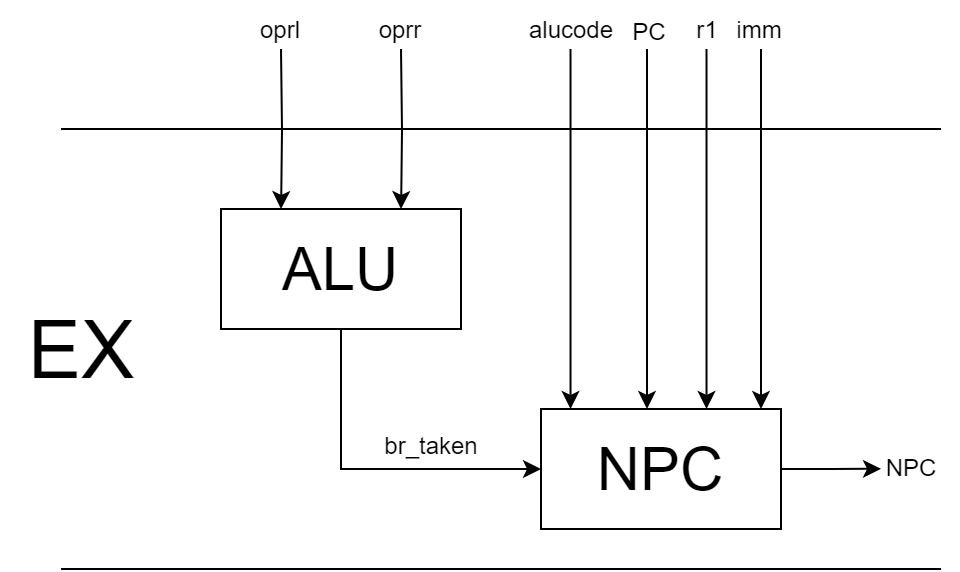
\includegraphics[width=7.5cm]{figure/NPC1.png}
        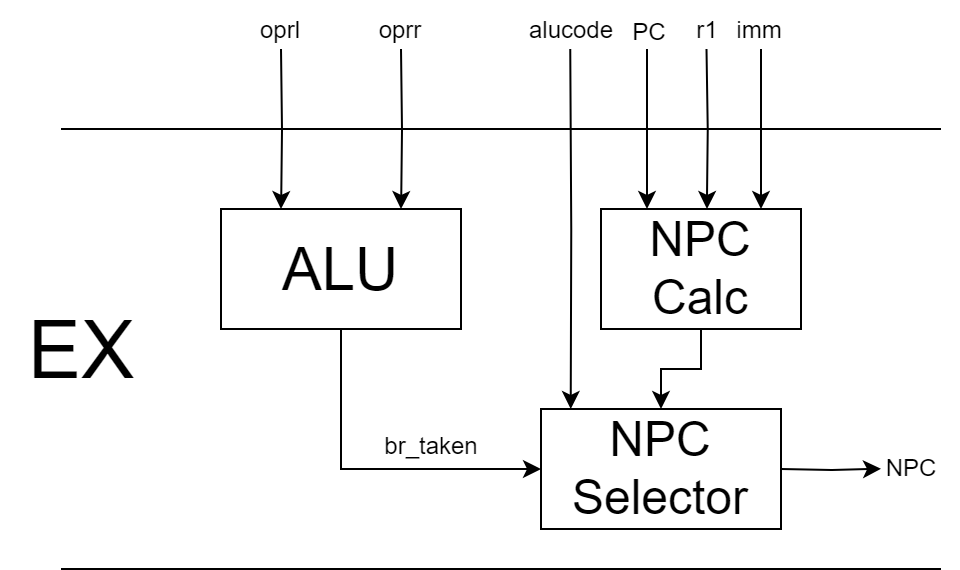
\includegraphics[width=7.5cm]{figure/NPC2.png}
        \caption{EXステージ}\label{fig:NPC}
    \end{figure}

    次なるクリティカルパスとして、MAステージに注目した。
    v3.1のアーキテクチャでは、クロックの立ち上がりでEXステージからMAステージにデータを渡し、RAMの読み書きがあればクロックの立ち下がりで行う。
    立ち下がりの処理は重く、次のクロックの立ち上がりまでに計算しなければいけないため、クリティカルパスとなっていた。
    そこで図~\ref{fig:clkduty}のように、クロックのDuty比をVivado上で5:5から4:6に変更し、RAMの読み書きに使える時間を増やすことで解消を試みた。
    \begin{figure}[h]
        \centering
        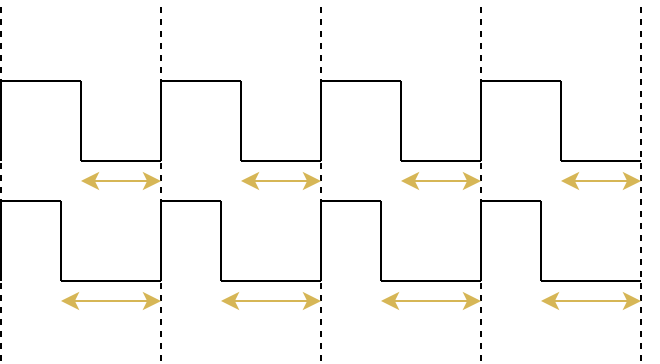
\includegraphics[width=12cm]{figure/clock_duty.png}
        \caption{クロックのDuty比}\label{fig:clkduty}
    \end{figure}
    更に最終的には、RAMの読み書きのフラグやアドレスをパイプラインレジスタ経由でなく演算結果をそのまま用いることで、RAMの読み書きをクロックの立ち上がりで行うようにした。
    \subsubsection{パフォーマンス}
    Vivadoを用いて合成したところ、最大クロック周波数は$90\mathrm{MHz}$付近となった。
    FPGA上で$90\mathrm{MHz}$でCoreMarkを動作した結果は表~\ref{tab:v3.2}の通りである。
    \begin{table}[h]
        \begin{center}
            \caption{v3.2のCoreMark結果}\label{tab:v3.2}
            \begin{tabular}{ll}
                CoreMark & 105\\
                CoreMark / MHz & 1.17 \\
                IPC & 0.849 \\
                分岐成功率 & 93.85\% \\
            \end{tabular}
        \end{center}
    \end{table}
    当初の目標であるCoreMarkスコア3桁を達成した。
    \subsection{v4.0}
    \subsubsection{実装内容}
    v3.2までのプロセッサでは原理上IPCが1までしか上がり得ず、
    ここまでの実験結果から$F[\mathrm{MHz}] \times \mathrm{IPC}\times 1.4$付近がCoreMarkスコアの上限であると予想した。
    これ以上CoreMarkスコアを大きく向上させるためには命令レベル並列処理を行うか、対応する命令を増やす必要がある。v4台ではRV32M命令を実装した。

    CoreMarkのIterationには``list\_join'', ``matrix'', ``state''の3つがあり、うち``matrix''は行列演算のタスクで、たくさんの積和演算からなる。
    RV32Iでは乗算を行う命令がないため、Listing~\ref{lst:matrix}のようにビット演算と加算の組み合わせで32bitの積を計算している。
    \lstinputlisting[caption=CoreMarkの積の実装,label=lst:matrix]{code/mul.asm}
    これは最悪ケースで約200クロックを消費するうえ、中で行う分岐は乗数の値によって変化するため、分岐予測が難しい。
    また、乗数・被乗数のレジスタが$\mathrm{a0}, \mathrm{a1}$で固定されており、いちいちmv命令でレジスタを移動する必要がある。

    この部分をRV32M命令の乗算命令に置き換えることで無駄を省くことができ、計算の大幅な高速化が可能であると考えた。

    これらを1クロックで計算しようとするとクロック周波数が大幅に下がってしまうため、複数クロックで計算する乗除算器を実装した。
    \begin{figure}[h]
        \centering
        \includegraphics[width=7cm]{figure/mul.png}
        \caption{乗算の計算方法}\label{fig:multiplier}
    \end{figure}
    \begin{figure}[h]
        \centering
        \includegraphics[width=10cm]{figure/divrem.png}
        \caption{除算の計算方法}\label{fig:divrem}
    \end{figure}
    乗算器は図~\ref{fig:multiplier}、除算器は図~\ref{fig:divrem}のように、2進数の筆算を行うように実装した。
    1クロックに付き1bitずつ計算を行う。
    前処理として1クロックで符号なしへの変換と、最上位ビットの符号拡張を行い、後処理として1クロックで符号付きへの変換を行うので、計34クロックで乗算・除算が完了する。

    EXステージで処理している命令が乗算・除算命令の場合、ALUの代わりに乗除算器を使い、その間他のステージの処理はストールさせる。
    \subsubsection{パフォーマンス}
    Vivadoを用いて合成したところ、最大クロック周波数は$90\mathrm{MHz}$付近となった。
    FPGA上で$90\mathrm{MHz}$でCoreMarkを動作した結果は表~\ref{tab:v4.0}の通りである。
    \begin{table}[h]
        \begin{center}
            \caption{v4.0のCoreMark結果}\label{tab:v4.0}
            \begin{tabular}{ll}
                CoreMark & 142\\
                CoreMark / MHz & 1.58 \\
                IPC & 0.454 \\
                分岐成功率 & 98.38\% \\
            \end{tabular}
        \end{center}
    \end{table}
    CoreMarkスコア、分岐予測率の向上が見られた。
    \subsection{v4.1}
    \subsubsection{実装内容}\label{sec:v4.1}
    v4.1では、v4.0の乗算器を改良した。
    $A\times B$を計算するとき、Bをいくつかに分割してそれぞれ積を求め、それらの積を足し合わせることで計算しても良い。
    そこで、図~\ref{fig:multiplier2}のようにBを4bitずつ8個に分割し、それぞれを同時に処理する(4クロック)
    これら8つの和を2クロックかけて足し合わせることで$A\times B$を計算する。
    これにより、乗算器の処理時間を34クロックから8クロックに短縮した。
    さらに、Bの8分割は連続する4bitずつに分ける必要はないので、
    \begin{itemize}
        \item 1クロック目: B[7:0]を処理
        \item 2クロック目: B[15:8]を処理
        \item 3クロック目: B[23:16]を処理
        \item 4クロック目: B[31:24]を処理
    \end{itemize}
    というように分けることで、乗数が小さい場合は更に短いクロックで計算を切り上げられるようにした。
    \begin{figure}[h]
        \centering
        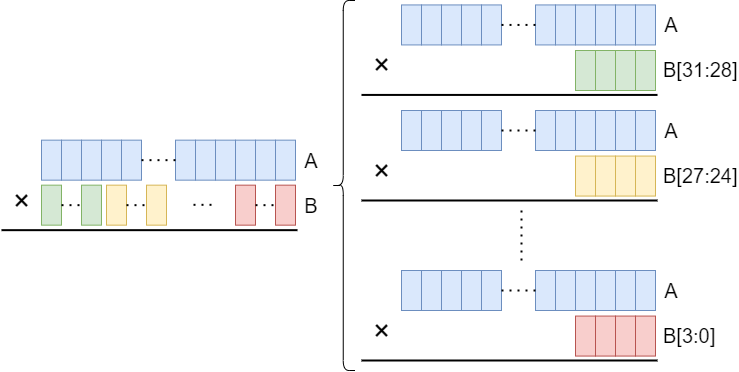
\includegraphics[width=12cm]{figure/mul_split.png}
        \caption{乗算の並列化}\label{fig:multiplier2}
    \end{figure}

    除算・剰余に対しても1クロックに数桁分まとめて処理することで高速化することができるが、CoreMarkのIterationでは除算・剰余の計算が少なく
    パフォーマンスにはあまり影響しなかったため、実装しなかった。

    \subsubsection{パフォーマンス}
    Vivadoを用いて合成したところ、最大クロック周波数は$90\mathrm{MHz}$付近となった。
    FPGA上で$90\mathrm{MHz}$でCoreMarkを動作した結果は表~\ref{tab:v4.1}の通りである。
    \begin{table}[h]
        \begin{center}
            \caption{v4.1のCoreMark結果}\label{tab:v4.1}
            \begin{tabular}{ll}
                CoreMark & 250\\
                CoreMark / MHz & 2.78 \\
                IPC & 0.780 \\
                分岐成功率 & 98.38\% \\
            \end{tabular}
        \end{center}
    \end{table}

    \section{まとめ}
    \subsection{取り組んだこと・取り組まなかったこと}
    本実験では、最終的にCoreMarkスコア250を達成した。
    最終的なアーキテクチャで実装した機能は以下の通りである。
    \begin{itemize}
        \item RV32I命令セット
        \item 5ステージパイプライン
        \item 分岐予測器(BTB, PHT)
        \item RV32M命令セット(および乗算の高速化)
    \end{itemize}
    また、最終的なアーキテクチャで実装しなかった機能は以下の通りである。
    \begin{itemize}
        \item 高度な分岐予測:
        2bitのPHTでは、for文の終了判定などの分岐を正しく予測できない。ローカル履歴やグローバル履歴を用いた分岐予測器を実装することで、分岐予測率を向上させることができる。
        グローバル履歴を用いた分岐予測器としてgshareがある。PHTのインデックスにPCの下位ビットを用いるのではなく、PCの下位ビットと過去の分岐履歴をXORした値をインデックスとするもので、
        分岐履歴を考慮した分岐予測が可能である。
        今回gshareを実装したものの、CoreMarkパフォーマンスは向上しなかった。
        理由として、CoreMarkでは単純な分岐が多く既に十分な精度が出ていたこと、PHTのインデックスが256と小さく、むしろインデックスの衝突が増えてしまったことが考えられる\footnote{\url{https://lpha-z.hatenablog.com/entry/2020/03/08/231500}}。
        \item DSPを用いた乗算の高速化:
        今回用いたFPGA上にはDSPと呼ばれる乗算器があり、これを用いることで乗算を高速化することができる。
        Vivadoには、DSPを用いて乗算をパイプライン化\footnote{\url{https://docs.xilinx.com/r/ja-JP/ug901-vivado-synthesis}}
        する機能があり、これは自力で実装するよりも高速に動作するはずである。
        \item 除算の高速化: 
        \ref{sec:v4.1}で述べたように、除算も乗算と同様に高速化することができるが、CoreMarkスコアに影響がなかったため実装しなかった。
        \item スーパスカラ: 
        今回のプロセッサは1クロックに1命令しか実行できないが、1クロックに複数命令を実行できるスーパスカラプロセッサを実装することで、IPCを向上させることができる。
        しかしながら、考慮しなければいけない命令の依存関係が爆発的に増加する。もっとも初歩的なスーパースカラとして、PC+4の命令をフェッチ・デコードし、
        PC, PC+4ともにOP命令で、RAW依存関係がない場合に限り実行するものを検討した。しかしながら、このケースであっても
        一個前のEXステージ・MAステージからフォワーディングの可能性があり、
        フォワーディング元(EX1, EX2, MA)、フォワーディング先(EX1のoprl, oprr, EX2のoprl, oprr)で12パターンの依存関係を考慮しなければいけない。
        これを実装するには各ステージの機能がカプセル化されていて、それらの結合が簡潔に記述されていないと難しいと考え、実装を断念した。
    \end{itemize}
    \subsection{CoreMarkスコア推移}
    実験開始からの経過日数とCoreMarkスコアの推移を図~\ref{fig:score}に示す。
    \begin{figure}[h]
        \centering
        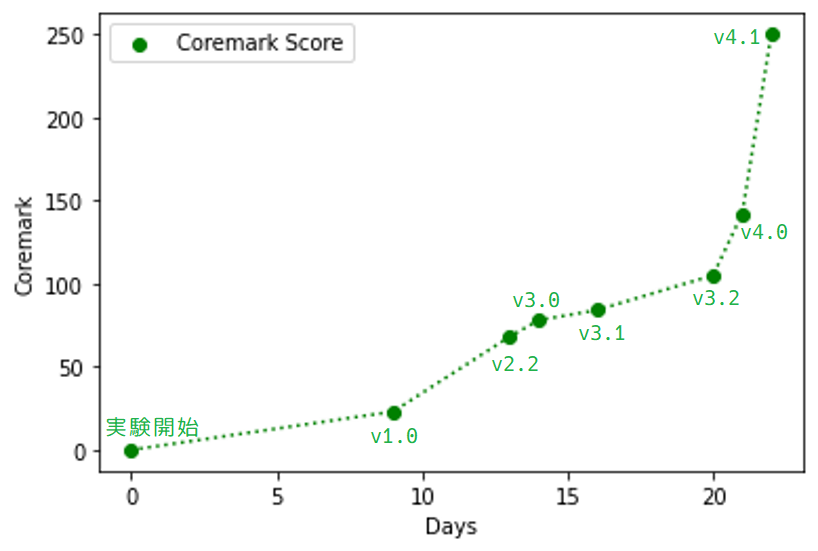
\includegraphics[width=12cm]{figure/coremark_plot.png}
        \caption{CoreMarkスコアの推移}\label{fig:score}
    \end{figure}
    全体を通してクロック周波数は大きく変化していないため、IPCの向上がCoreMarkスコアに直結した。
    効果が大きかったのは、パイプライン化(IPC最大5倍)と乗算器の高速化(乗算・20倍以上)であった。
    分岐予測も効果はあったが、予測率の向上はたかだか数割なのでCoreMarkスコアが劇的に向上することはなかった。RV32M命令よりも先に実装していて良かったと思う。
    \subsection{感想}
    今回の実験はかなり楽しく、実験時間外でもかなりの時間を費やした。
    ちょっと記法や構造を変えるだけでパフォーマンスが大きく変わり、試行錯誤しがいがあった。
    また、同じ機能を実装しても人によって実装・動作周波数・スコアが大きく異なるため、色々な人と議論や情報共有をしながら進めることができるのもよかった。

    最後にスーパースカラを実装できなかったことが残念である。モジュールの整理・全体のリファクタリングが不十分だったように思う。
    しかし、当初掲げていた目標であるCoreMarkスコア3桁を達成でき、開発自体はとても順調だったので、満足している。
\end{document}